% --- Chapter 2: System Design ---
\chapter{Проектування системи}
\label{ch:design}

\section{Функціональні та нефункціональні вимоги}
\label{sec:requirements}
Проектування веб-застосунку \textit{Beekeepers Community Platform} базувалося на визначенні ключових функціональних та нефункціональних вимог, що забезпечують його корисність, надійність та зручність для користувачів.

\subsection{Функціональні вимоги}
\begin{itemize}
    \item \textbf{Реєстрація та автентифікація користувачів:} Можливість створення облікового запису з використанням електронної пошти та паролю, верифікація email через надсилання підтверджувального листа, а також автентифікація за допомогою облікового запису Google (OAuth 2.0).
    \item \textbf{Управління профілем користувача:} Перегляд та редагування базової інформації профілю (наприклад, біографія, місцезнаходження, експертиза).
    \item \textbf{Форум для обговорень:} Створення нових тем для обговорення, публікація повідомлень у темах, можливість залишати коментарі до повідомлень, система вподобань (лайків) для постів.
    \item \textbf{База знань:} Доступ до каталогу статей та ресурсів з бджільництва, можливість пошуку та фільтрації матеріалів за категоріями (поточна реалізація з mock-даними).
    \item \textbf{Інтерактивна карта (Управління пасіками та полями):} 
        \begin{itemize}
            \item Відображення карти (Україна за замовчуванням).
            \item Додавання точкових маркерів для вуликів із зазначенням назви та нотаток.
            \item Додавання полігональних об'єктів для полів із зазначенням назви, типу культури, періоду цвітіння та запланованих дат обробки пестицидами/інсектицидами.
            \item Перегляд, редагування (заплановано) та видалення (заплановано) маркерів та полігонів.
            \item Відображення детальної інформації (метаданих) при виборі об'єкта на карті.
            \item Фільтрація об'єктів на карті за різними критеріями (тип культури, період цвітіння для полів; тип вулика, стан для пасік).
            \item Можливість отримання сповіщень про заплановані обробки полів поблизу пасік (майбутній функціонал).
        \end{itemize}
    \item \textbf{Інтернаціоналізація:} Підтримка декількох мов інтерфейсу (українська, англійська).
\end{itemize}

\subsection{Нефункціональні вимоги}
\begin{itemize}
    \item \textbf{Продуктивність:} Забезпечення прийнятного часу завантаження сторінок та швидкої відповіді сервера на запити користувачів.
    \item \textbf{Безпека:} Захист облікових записів користувачів (хешування паролів), валідація вхідних даних на клієнті та сервері, використання HTTPS у продакшн-середовищі, захист від поширених веб-вразливостей (наприклад, XSS через використання React, який екранує дані за замовчуванням).
    \item \textbf{Масштабованість:} Архітектура застосунку повинна дозволяти майбутнє масштабування для обслуговування зростаючої кількості користувачів та обсягів даних.
    \item \textbf{Надійність:} Система повинна бути доступною та стабільно працювати.
    \item \textbf{Зручність використання (Usability):} Інтерфейс має бути інтуїтивно зрозумілим, легким у навігації та адаптивним для різних розмірів екранів (десктоп, мобільні пристрої).
    \item \textbf{Підтримуваність коду:} Кодова база повинна бути добре структурованою, документованою (де необхідно) та легкою для модифікації та розширення.
\end{itemize}

\section{Діаграми варіантів використання (Use Case Diagrams)}
\label{sec:use_cases}
% TODO: Create Use Case diagrams for major actors (Unregistered User, Registered User, Admin (if any)).
% Example:
% \begin{figure}[H]
%   \centering
%   \includegraphics[width=0.8\textwidth]{images/use_case_diagram.png} % Replace with your actual diagram
%   \caption{Діаграма варіантів використання для зареєстрованого користувача}
%   \label{fig:use_case_registered_user}
% \end{figure}
Тут мають бути представлені діаграми варіантів використання, що ілюструють взаємодію користувачів (акторів) із системою. Наприклад, для незареєстрованого користувача (перегляд публічного контенту, реєстрація), зареєстрованого користувача (вхід, участь у форумі, робота з картою, перегляд бази знань, управління профілем) та адміністратора (якщо передбачено).

\section{Архітектура системи}
\label{sec:architecture}
Розроблений веб-застосунок має класичну клієнт-серверну архітектуру. 

\subsection{Загальна архітектура}
Система складається з трьох основних компонентів: 
\begin{itemize}
    \item Клієнтська частина (Frontend): односторінковий застосунок (SPA), розроблений на React, відповідає за користувацький інтерфейс та взаємодію з користувачем.
    \item Серверна частина (Backend): REST API, розроблене на NestJS, відповідає за бізнес-логіку, обробку запитів, взаємодію з базою даних та автентифікацію.
    \item База даних: MongoDB, документо-орієнтована NoSQL база даних, використовується для зберігання всієї інформації застосунку, включаючи дані користувачів, пости форуму, статті бази знань, а також геопросторові дані для карти.
\end{itemize}
Взаємодія між клієнтом та сервером відбувається за протоколом HTTP(S) через RESTful API. Для розгортання використовується Docker, що забезпечує ізоляцію та портативність середовища.
% \begin{figure}[H]
%   \centering
%   % 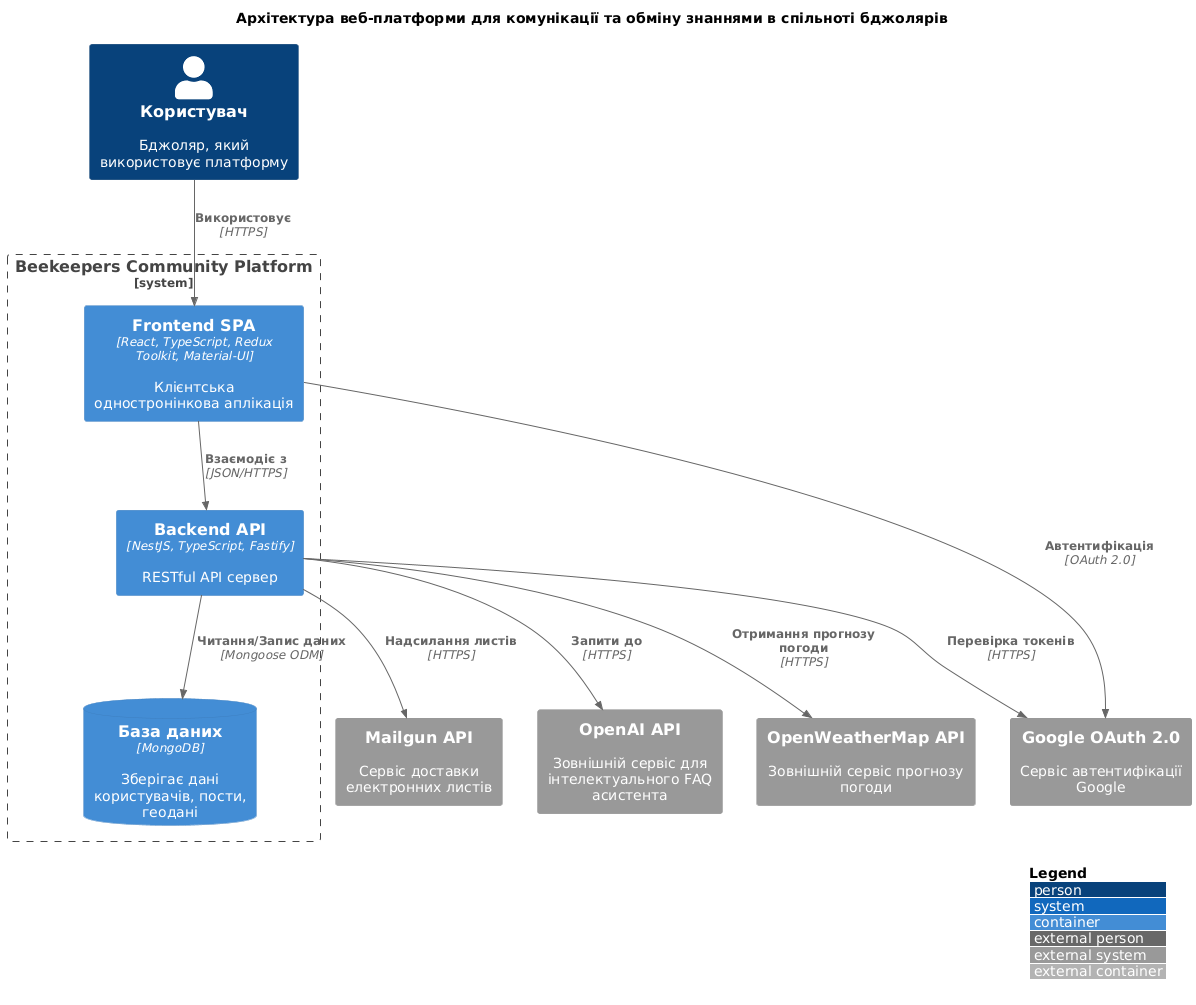
\includegraphics[width=0.7\textwidth]{images/system_architecture.png} % TODO: Add actual diagram
%   \fbox{Placeholder for High-Level System Architecture Diagram}
%   \caption{Загальна архітектура системи}
%   \label{fig:system_architecture}
% \end{figure}

\subsection{Архітектура фронтенду}
Клієнтська частина розроблена з використанням бібліотеки React та TypeScript. Управління станом реалізовано за допомогою Redux Toolkit, зокрема RTK Query для взаємодії з API та кешування даних. Навігація між сторінками забезпечується React Router. Для побудови користувацького інтерфейсу використано бібліотеку компонентів Material-UI (MUI), що дозволяє створювати адаптивні та візуально привабливі інтерфейси. Інтернаціоналізація реалізована за допомогою i18next та react-i18next. Картографічний функціонал побудований на базі Leaflet та React-Leaflet.
Структура проекту включає розділення на компоненти (загального призначення та специфічні для функціоналу), сторінки, сервіси (API-зрізи RTK Query), хуки, контексти та утиліти.

\subsection{Архітектура бекенду}
Серверна частина розроблена на платформі Node.js з використанням фреймворку NestJS та TypeScript. Архітектура є модульною, де кожен функціональний блок (наприклад, автентифікація, користувачі, форум, карта) виділений в окремий модуль. Кожен модуль містить контролери (обробка HTTP-запитів), сервіси (бізнес-логіка) та DTO (Data Transfer Objects) для валідації вхідних даних. Для взаємодії з базою даних MongoDB використовується ODM Mongoose. Автентифікація реалізована за допомогою Passport.js (JWT, локальна стратегія, Google OAuth). Для автоматичної генерації документації API використовується Swagger (OpenAPI). Застосунок працює на базі веб-сервера Fastify для підвищення продуктивності.

\subsection{Схема бази даних}
База даних MongoDB зберігає дані у вигляді колекцій документів. Основні колекції включають:
\begin{itemize}
    \item \texttt{users}: інформація про користувачів (email, хеш паролю, ім'я користувача, профільні дані, статус верифікації, токени, геодані тощо).
    \item \texttt{forumposts}: пости на форумі (заголовок, зміст, автор, коментарі, лайки).
    \item \texttt{hives}: дані про вулики (назва, нотатки, геокоординати GeoJSON Point, власник).
    \item \texttt{fields}: дані про поля (назва, тип культури, періоди цвітіння та обробки, геометрія GeoJSON Polygon, власник).
    \item (Інші колекції, якщо є, наприклад, для бази знань, подій).
\end{itemize}
Для геопросторових даних (координати вуликів та геометрія полів) використовуються відповідні індекси \texttt{2dsphere} для ефективних геозапитів.
% \begin{figure}[H]
%   \centering
%   % 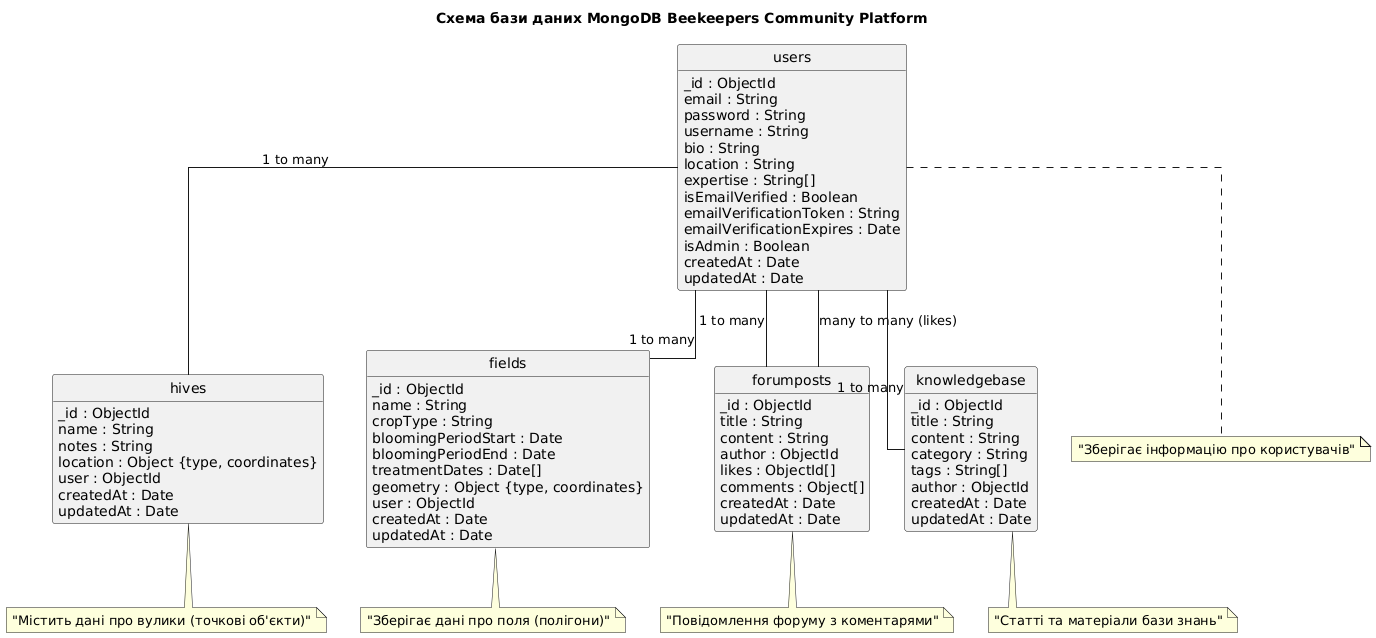
\includegraphics[width=\textwidth]{images/db_schema.png} % TODO: Add actual ERD/schema diagram
%   \fbox{Placeholder for Database Schema Diagram}
%   \caption{Логічна схема бази даних}
%   \label{fig:db_schema}
% \end{figure}

\section{Проектування UI/UX}
\label{sec:ui_ux}
Проектування користувацького інтерфейсу (UI) та досвіду взаємодії (UX) було спрямоване на створення інтуїтивно зрозумілої, зручної та візуально привабливої платформи. Основним інструментом для реалізації UI стала бібліотека компонентів Material-UI, яка надає широкий набір готових елементів дизайну, що відповідають сучасним стандартам Material Design. 

Ключові рішення:
\begin{itemize}
    \item \textbf{Адаптивний дизайн:} Забезпечення коректного відображення та функціонування на різних пристроях (десктопи, планшети, мобільні телефони).
    \item \textbf{Інтуїтивна навігація:} Використання бічної панелі навігації для доступу до основних розділів сайту та чіткої ієрархії сторінок.
    \item \textbf{Консистентність інтерфейсу:} Дотримання єдиного стилю оформлення елементів на всіх сторінках застосунку.
    \item \textbf{Інтерактивність:} Надання користувачам можливості легко взаємодіяти з елементами, такими як карта, форми, кнопки.
    \item \textbf{Зворотний зв'язок:} Інформування користувача про результати його дій (успіх, помилка, процес завантаження) за допомогою повідомлень та індикаторів.
\end{itemize}
% TODO: Include wireframes or mockups if available (can be in appendix). 

\subsubsection{Вимоги до форуму}
\begin{itemize}
    \item Реєстрація користувачів з верифікацією електронної пошти.
    \item Автентифікація (логін/пароль, можливість входу через Google OAuth).
    \item Зберігання даних користувачів (email, хеш паролю, ім'я користувача, роль, інформація про пасіку за бажанням).
    \item Управління профілем користувача.
    \item Відновлення паролю.
\end{itemize}

\subsubsection{Вимоги до бази знань}
\begin{itemize}
    \item Створення, редагування та видалення статей/ресурсів адміністраторами.
    \item Категоризація та тегування матеріалів.
    \item Пошук по базі знань.
    \item Система коментарів до статей (за бажанням).
    \item Рейтинг статей (за бажанням).
\end{itemize}

\subsubsection{Загальні нефункціональні вимоги}
\begin{itemize}
    \item \textbf{Безпека:} Захист від основних веб-вразливостей (XSS, CSRF, SQL/NoSQL ін'єкції), безпечне зберігання паролів, використання HTTPS.
    \item \textbf{Продуктивність:} Швидке завантаження сторінок та відгук інтерфейсу.
    \item \textbf{Масштабованість:} Архітектура повинна дозволяти додавання нового функціоналу та витримувати зростання кількості користувачів.
    \item \textbf{Надійність:} Система повинна бути доступною та стабільно працювати.
    \item \textbf{Зручність використання (Usability):} Інтуїтивно зрозумілий та легкий у використанні інтерфейс.
    \item \textbf{Адаптивність (Responsiveness):} Коректне відображення на різних пристроях (десктопи, планшети, мобільні телефони).
    \item \textbf{Інтернаціоналізація (i18n):} Підтримка української та англійської мов інтерфейсу.
    \item \textbf{Зворотний зв'язок:} Інформування користувача про результати його дій, помилки.
\end{itemize} 